\vfill\pagebreak


\section{Hardware setup and event data\label{sec:Hardware-setup-and}}

This section describes the hardware setup and gives an intuition of
the event data that a DVS produces.


\subsubsection{DVS and its interface\label{sec:interface}}

The DVS attaches to a computer using a common USB port. The camera
is distributed with a portable software framework written in Java
called jAER~\cite{jaer}. This project, developed in C++ for maximum
efficiency, needed a special driver to be developed, based on the
Thesycon USB device driver~\cite{thesycon}. The events are transmitted
from the camera in packets of up to several hundred events; however,
each event is independently tagged at the source with its proper timestamp.



\subsubsection{Active LED Markers (\ALMs)\label{sec:leds}}

The LED controller is based on the bronze board~\cite{bronzeboard}
from inilabs, which is based on an AVR32.  We used infrared LEDs
since the DVS is most sensitive in the infrared spectrum. 



In our setup we could easily change the PWM frequency to the LEDs.
An upper bound on the detectable frequency depends on the power of
the LEDs and the distance to the camera; a DVS camera is not magic:
there must be a large enough change in the number of photons reaching
the photoreceptor to trigger an event. In our setup we found 2~KHz
to be an adequate number. The frequencies for each LEDs were then
decided in the interval 1--2~KHz making sure we did not choose frequencies
with common harmonics. A reasonable lower bound on the blinking frequency
was found experimentally to be $1$~KHz to minimize the confusion
between with background motion (see \prettyref{sub:Alternate-events-and-motion}
below).


\subsubsection{Statistical properties of event sequences}

\begin{figure}[b]
\begin{centering}
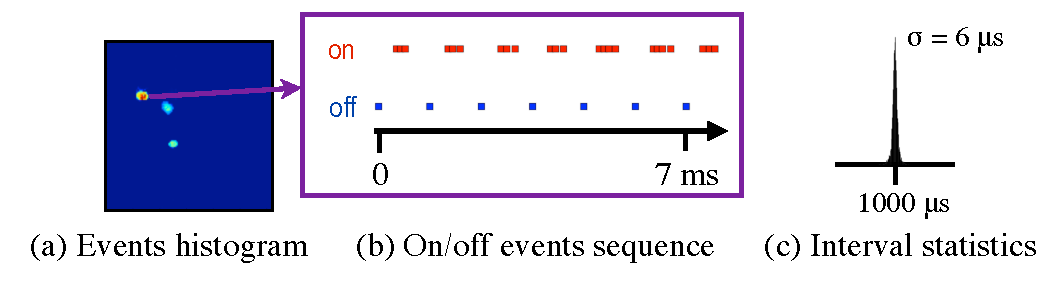
\includegraphics[width=9cm]{figures/slides/event_sequence2}
\par\end{centering}

\caption{\label{fig:events-hist}Example event sequence from a DVS looking
at an Active LED Marker (\ALM). Subfigure (a) shows the histogram
of events seen from a fixed camera looking at three \ALMs. The difference
in numbers is due to the different frequencies of the \ALMs. Subfigure
(b) shows a slice of the events seen at a particular pixel near the
center of one of the \ALMs which has a blinking frequency of 1 KHz.
The data is a series of events with positive (\pP) and negative (\pN)
events. (c) The sequence of \pPN transitions are highly regular;
in this data we observed that the distribution of the intervals is
well approximated by a Gaussian with mean $1000\,\mu s$ and standard
deviation $\sigma=6\,\mu s$. }
\end{figure}


\prettyref{fig:events-hist} gives an intuition of how the data looks
like. In this scenario both the \ALMs and the DVS are fixed. \prettyref{fig:events-hist}\emph{a}
shows the histogram of the number of events coming from a particular
pixels. The three peaks are the three \ALMs ($f=500,700,1000\,\mbox{Hz}$).
The number of events is different for each peak because the frequencies
differ. The halo in \prettyref{fig:events-hist}\emph{a} cannot be
explained by the refractive properties of the optics, and is probably
due to non-ideal local interactions among neighbors in the sensing
array.

\prettyref{fig:events-hist}\emph{b} shows the sequence of events
obtained from one particular pixel, corresponding to an \ALM  with
a frequency of 1~KHz. There is a different number of P and N events,
which tells us that we cannot really interpret the DVS data as simply
the derivative of the image. 

For this particular data, the P events arrive noisily, while the N
events arrive more regularly. Note that the what we observe here is
the combination of the LED dynamics with the dynamics of the photoreceptor
and the nonlinear detector. Experimentally we found that the interval
between successive P/N transitions is repeatable: we have observed
that the jitter is well approximated by a Gaussian with standard deviation
equal to $6\,\mu s$ (\prettyref{fig:events-hist}\emph{c}).


\subsubsection{Effect of motion\label{sub:Alternate-events-and-motion}}

\begin{figure}[b]
\centering{}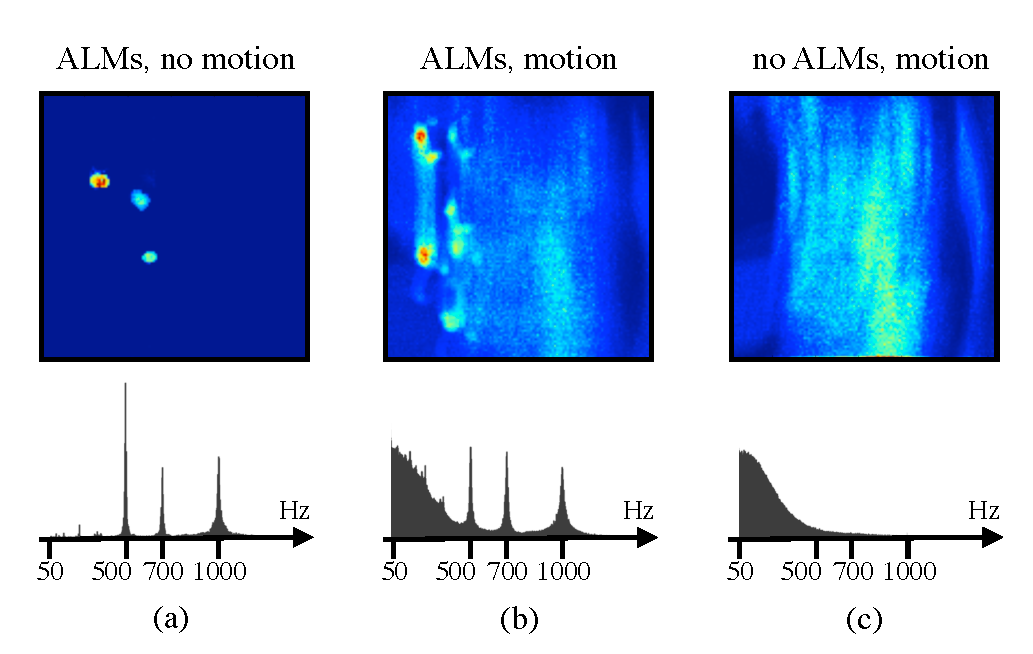
\includegraphics[width=8.6cm]{figures/slides/motion}\caption{\label{fig:switch-hist}Comparison of transition events statistics
in three cases: a)~visible markers, without motion; b)~with camera
motion; c)~with camera motion but no marker visible. Note in (c)
that the motion of the camera creates apparent motion of the environment
and a large number of events; however they are of a low frequency.
In this case, the events from the background are negligible after
$700$~Hz, though this depends on the statistics of the environment
and the speed of the motion. We can choose the frequencies of the
markers high enough such that they are not confused as background
motion.}
\end{figure}


Things get more complicated when the camera is moving, because the
apparent motion of the environment creates changes in luminance that
are unrelated to the \ALMs. However, we have found that we can discriminate
between the two types of events based on their temporal statistics.

\prettyref{fig:switch-hist} shows the histogram of frequencies of
the P/N transitions in three scenarios: a)~a fixed camera looking
at fixed \ALMs; b)~a moving camera looking at fixed \ALMs; c)~a
moving camera with no LEDs. From this data we can see that the motion
of the camera generates a large number of events, but at low frequencies,
and notwithstanding the motion, we can still clearly see the peaks
originated from the markers. Therefore, if we choose the marker frequencies
high enough, we can filter for the camera motion just by ignoring
the events corresponding to frequencies under a certain threshold. 
